\chapter{Freedom Inside the Constraints}

A system that builds the next instance of itself seems to offer a way around the manufacturing bottleneck. A simulated world seems to offer a way around the burden of physical experience. Both are useful stress tests for the book's argument. Where do resources, time, and coupling go when the apparent route becomes so much lighter?

\section{Replication, Irreversibility, and the Substrate}

\subsection{What Self-Replication Changes}

Compare a fixed production line with an idealized population that doubles at a constant interval:
\begin{equation}
 N_{\mathrm{line}}(t)=1+\frac{t}{\tau_{\mathrm{line}}},
 \qquad
 N_{\mathrm{rep}}(t)=2^{t/\tau_{\mathrm{rep}}}.
\end{equation}
The quantities are unit counts relative to the stated starting condition. The first assumes fixed capacity; the second assumes adequate inputs and an unchanged doubling time. A manufacturing system can add capacity, and a replicating system can encounter limits. The assumptions define the comparison.

Replication can distribute construction. It still needs feedstock, energy, space, transport, error control, and waste handling. The next producer is also something that must be built and maintained.

The resource barrier becomes an uptake problem: what can be extracted or obtained from the environment at the required rate? The temporal constraint includes the cycle of acquisition, construction, maturation, and copying. The topology includes access to suitable environments and pathways of spread.

None of these is intrinsically faster than every manufacturing process. Biological replication can be fast for a microbe and slow for a tree. An engineered replicator's rate would depend on what it must reproduce and the environment it assumes.

Von Neumann's formal construction demonstrated a way to separate a description, its copying, and its use by a constructor \cite{vonneumann1966theory}. Physical implementation adds a full industrial and thermodynamic account. A printer making one of its own parts is a useful step toward automation; it is not yet an autonomous system rebuilding its entire supply basis.

The governance problem changes when production is dispersed beyond a few facilities. Monitoring spread, limiting access to necessary conditions, and preserving effective intervention points can become more important. Their effectiveness must be established for the particular system.

The ratio
\begin{equation}
 \chi=\frac{\tau_{\mathrm{assessment}}}
            {\tau_{\mathrm{doubling}}}
\end{equation}
identifies one timing pressure. Under continued ideal doubling, assessment lasting $\chi$ doubling times permits a factor $2^\chi$ increase before completion. A large ratio can make delayed recognition costly. Containment, access, detection quality, and intervention strength still determine whether control is possible.

\subsection{Growth Can Settle, Oscillate, or Overshoot}

Exponential growth cannot continue indefinitely in a finite environment. Its eventual form depends on the feedback.

A delayed logistic model illustrates the difference:
\begin{equation}
 \frac{\mathrm dN}{\mathrm dt}
 =rN(t)\left(1-\frac{N(t-\theta)}{K}\right).
\end{equation}
$r>0$ is a growth rate, $K>0$ a fixed capacity, and $\theta$ a feedback delay. The state requires an initial history over the delay interval.

Linearizing around the positive equilibrium $N=K$ gives
\begin{equation}
 \dot u(t)=-r\,u(t-\theta).
\end{equation}
For this model, the equilibrium is locally asymptotically stable when $r\theta<\pi/2$, with the first stability boundary at $r\theta=\pi/2$. Beyond that boundary, the local equilibrium loses stability. The full nonlinear behavior requires further analysis.


\begin{figure}[ht]
\centering
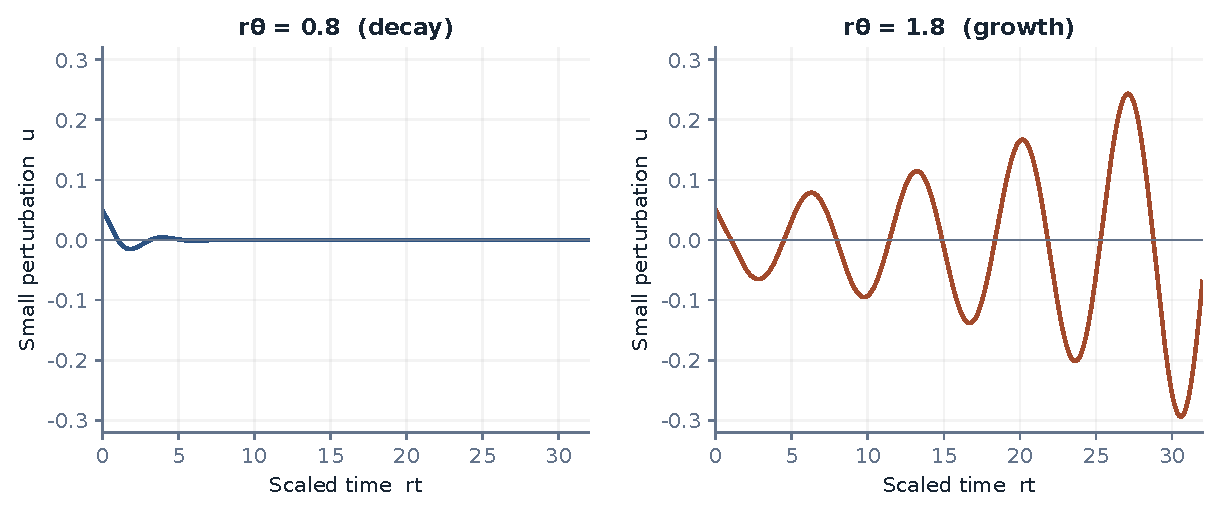
\includegraphics[width=\textwidth]{assets/delay-stability.pdf}
\caption{Linearization of the delayed logistic model near its positive equilibrium gives $\dot u=-ru(t-\theta)$. Numerical illustrations start from a small constant history. Perturbations decay at $r\theta=0.8$ and grow at $r\theta=1.8$; the first local stability boundary is $\pi/2$. These are local linear dynamics.}
\label{fig:mechanism-delay-stability}
\end{figure}
Regulated growth can settle. Delays can create oscillation. Environmental damage can reduce capacity. A richer model may need resource and waste variables as well as population.

The physical challenge is to design and maintain effective feedback before the receiving environment has changed too much. The same concern appears in ordinary manufacturing, though replication can distribute and amplify it differently.

Self-replication relocates a bottleneck toward ecological relations. It keeps the resource, time, and network questions alive.

\subsection{Consequential Weight Depends on the Task}

A reversible operation can be physically real. A draft can be deleted and still have consumed energy, time, and attention. Irreversibility therefore measures aspects of consequence; it is not a complete test for existence.

The practical question is which history remains relevant to later action. A version-controlled file can be restored. A disclosure to another person cannot be fully recalled. A simulation can reset its internal state while its user's learning persists.

The same representation can cross several boundaries. A fictional story may change a relationship. A simulated experiment may guide a real intervention. The carrier's reversibility does not settle the reversibility of its effects.

This is why a useful account specifies scale, boundary, and horizon. It asks what the project can actually recover, rather than sorting everything into “virtual” and “real.”

\subsection{The Brain in a Vat Still Needs a Plant Room}

The familiar philosophical experiment supplies a brain with artificial experience. Its epistemological question is whether the subject could distinguish the arrangement from ordinary life.

The engineering question begins outside the experience: what keeps the brain functioning?

A living brain requires a carefully maintained environment with suitable supply, waste removal, temperature, chemistry, and physiological regulation. The power level of ordinary brain metabolism is on the order of tens of watts \cite{raichle2002}. An artificial support system would have its own additional bill.

Actual perfusion and preservation research investigates parts of the problem under specific conditions. It does not establish that a conscious human brain can be maintained indefinitely outside its body. Organ preservation, temporary support, restored cellular activity, and sustained personal experience are distinct endpoints.

A simple delivery relation can show the kind of constraint involved. For one supplied substance at a time,
\begin{equation}
 \dot Q\,\Delta C\geq\dot m,
\end{equation}
where $\dot Q$ is volume flow per unit time, $\Delta C$ usable concentration difference, and $\dot m$ consumption in matching mass or molar units. A separate linear hydraulic approximation gives
\begin{equation}
 \dot Q\leq\frac{\Delta p_{\max}}{R_{\mathrm h}}.
\end{equation}
The relations illustrate a possible supply-and-pressure window. Real cerebral circulation includes regulation, changing resistance, diffusion, tissue state, and multiple substances. They are not a clinical operating formula.

Heat also needs a destination. An operating biological or computational system must remain within the conditions its substrate tolerates. Better algorithms and cooling can reduce the burden, while thermodynamics still requires an adequate heat and entropy account.

The write-in interface adds another constraint. Electrode number, coding, correlation, noise, tissue response, and long-term stability affect what signals can be delivered or read. Research on implanted interfaces documents biological responses that influence performance \cite{polikov2005response}.

For $n$ ideal independent Gaussian channels of equal bandwidth $B$, a schematic capacity is
\begin{equation}
 C(t)=nB\log_2\left(1+\frac{S}{N(t)}\right).
\end{equation}
The result is bits per second. Actual neural interfaces do not automatically satisfy the assumptions, and useful experience cannot be inferred directly from a Shannon bit rate. Noise may change over time in either direction as tissue and hardware change.

Mapping a circuit is another achievement with its own boundary. The October 2026 connectome-based fly-model preprint couples a large measured wiring graph to a simulated body and tests sensorimotor behavior \cite{minnick2026sensorimotor}. It provides a current example of wiring, dynamics, and embodied feedback being studied together. A transferred human mind would require evidence of a different order.

The distinction becomes still sharper for a proposed substitution of biological neurons with artificial components. Functional equivalence, practical replaceability, preservation of continuity, and consciousness would each need evidence or a separate argument. The engineering operation is hypothetical.

Even a successful substitution would change the substrate rather than abolish it. The new system would have some requirements for energy, temperature, communication, maintenance, and repair.

Call this \emph{substrate inescapability}: every implemented process has a material support, and the support's properties enter what the process can sustain. The claim favors no particular material.

\subsection{The Outside Remains Part of the System}

A digital environment may permit resets while its servers age, its power supply depends on a grid, and its maintenance relies on people. A biological support system may create a carefully controlled interior while shifting complexity into pumps, chemistry, redundancy, and operations.

The interior's apparent simplicity can be a real benefit. The full comparison asks whether the external support costs are lower than the alternatives and how reliably they can be carried.

The same accounting applies to ordinary remote work and automated services. Removing a commute can save real resources. A data center, network, and maintenance organization add other requirements. Counting both reveals a possible net gain rather than assuming either a miracle or an exact transfer.

The two extremes converge on a concrete conclusion. Replication can distribute construction. Simulation can reorganize experience. Each still needs a working relation with a material environment.

Locating that relation gives design more freedom. It shows which conditions can be improved, which can be delegated, and which must remain protected for the process to continue.
